%! Author = joels
%! Date = 13/07/2021

\section{ASP.NET}
\subsection{C\# Grundlagen}
\begin{lstlisting}[style=csh]
// Anonyme Typen
var v = new { Amount = 108, Message = "Hello" };
// Keine Typechecks und kein IntelliSense
dynamic person = new ExpandoObject();
// Extension Method
public static class MyExtensions {
  public static int WordCount(this string str) { return
    str.Split(new char[] { ' ', '.', '?' }).Length; } }
// Middleware registrieren
app.Use(async (context, next) => {
  System.Diagnostics.Debug.WriteLine("Handling req.");
  await next.Invoke();
  System.Diagnostics.Debug.WriteLine("finish req"); });
// Verzweigung für Pfad
app.Map("/logging", builder => {
  builder.Run(async (context) => {
    await context.Response.WriteAsync("Hello"); }); });
// Request terminieren
app.Run(async (context) => {
  await context.Response.WriteAsync("Hello World!"); });
// Custom Middleware als Klasse (Wichtigste !!)
public class RequestLoggerMiddleware {
  public RequestLoggerMiddleware(RequestDelegate next, ILoggerFactory loggerFactory) {
    _next = next; _logger = loggerFactory.CreateLogger<RequestLoggerMiddleware>(); }
  public async Task Invoke(HttpContext context) {
    _logger.LogInformation("Handling request: " + context.Request.Path);
    await _next.Invoke(context); _logger.LogInformation("Finished handling request."); } }
\end{lstlisting}
\subsection{Dependency Injection}
ASP.NET Core kommt mit einem primitiven Dependency Injection Container. \textbf{Idee:} Klasse erwähnt welche Interfaces benötigt werden. Ein Resolver sucht im Container nach einer geeigneten Klasse und übergibt diese. \textbf{Ziel:} Reduzieren von hoher Kopplung zwischen verschiedenen Klassen.
\begin{lstlisting}[style=csh]
public class Startup {
  // called by runtime, Used to add services
  public void ConServices(IserviceCollection services) {
    services.AddTransient<IUserService, UserService>();}
  // Called by runtime, Configure HTTP req pipeline
  public void Configure(IApplicationBuilder app,
IHostingEnvironment env, ILoggerFactory loggerFactory) {
    app.UseMiddleware<UserMiddleware>(); } }
// Benutzen
public class UserMiddleware {
  private readonly RequestDelegate _next;
  public UserMiddleware(RequestDelegate next,
IUserService userService) { // Captive Dependency*
    _next = next; }
  public async Task Invoke(HttpContext context,
IUserService userService) { // No Captive Dependency
    await context.Response.WriteAsync(string.Join(", ", userService.Users)); } }
\end{lstlisting}
\textcolor{b}{\textbf{Transient:}} Created each time they are requested. Works best for lightweight, stateless services. \textcolor{b}{\textbf{Scoped:}} Created once per request. \textcolor{b}{\textbf{Singleton:}} Created the first time they are requested. Every subsequent request will use the same instance.\\
\textcolor{b}{\textbf{Captive Dependency Problematik:}} Komponenten dürfen sich nur Komponenten mit gleicher oder längerer Lebensdauer Injection lassen.
\subsection{Projekt-Struktur}
\textcolor{b}{\textbf{wwwroot:}} Statische Inhalte der Webseite z.B. CSS / JS / HTML
\textcolor{b}{\textbf{appsettings.json:}} Einstellungen der Webseite z.B. Connection-String zur DB
\textcolor{b}{\textbf{Programm.cs:}} Einstiegspunkt von der Web Applikation
\textcolor{b}{\textbf{Startup.cs:}} Konfiguriert die Web App
\subsection{Pages}
Alternative und vereinfachte Variante vom MVC. Router muss nicht konfiguriert werden. Best-Practices für Serverseitiges-Rendering. \textbf{Kombination mit MVC:} Statische Seiten mit Pages, REST-API mit MVC.\\
\textcolor{b}{\textbf{Routing:}} Bei Aufruf einer URL wird im Folder Pages gesucht $\rightarrow$ Ist case insensitive: \textcolor{b}{/add} rendert \textcolor{b}{/pages/add.cshtml}
\begin{lstlisting}[style=csh]
// View mit Razor File: *.cshtml
@page "/test/{id:int?}"
@model Examples.Pages.Page.RoutingModel
@{ ViewData["Title"] = "Routing"; }
<h1>Routing</h1>
<form asp-page="Bmi" data-ajax="true" data-ajax-method=
"POST"><input asp-for="@Model.Bmi.Height" name="height">
<button type="submit">submit</button></form>
// View Model File: *.cshtml.cs
public class RoutingModel : PageModel {
  // GET (Query)
  [BindProperty(SupportsGet = true)]
  public int Id { get; set; }
  // POST (Form)
  [BindProperty]
  public int Id2 { get; set; }
  // Hilfs-Methoden
  public void OnGet(){ ... }
  public void OnPost(){ ... } }
\end{lstlisting}
\subsection{Razor}
\textcolor{b}{\textbf{Shared/\_Layout.cshtml:}} Generelles Layout der App. Definierst Sections (Placeholders), welche von Page gefüllt werden.
\begin{lstlisting}[style=csh]
@RenderBody() // Platz für Content Page
@RenderSection("Nav", false); // Platz für Section Page
@section Nav{ /* ... */ }
\end{lstlisting}
\textcolor{b}{\textbf{\_ViewStart.cshtml:}} Hierarchisch, Code welcher vor Razor-Files ausgeführt wird. Definiert z.B. Layout für alle Pages
\begin{lstlisting}[style=csh]
@{ Layout = "_Layout"; }
\end{lstlisting}
\textcolor{b}{\textbf{\_ViewImports.cshtml:}} Hierarchisch, Namespaces / Tag-Helpers können in diesem File registriert werden.\\
\textcolor{b}{\textbf{Tag Helpers:}} Ermöglichen C\# Code an HTML Tags zu binden. Bsp: Email-Tag durch Link Tag ersetzen.
\begin{lstlisting}[style=csh]
<email mail-for="test@example.com"></email>
<a href="mailto:test@example.com">test@example.com</a>
public class EmailTagHelper : TagHelper {
  public string MailFor { get; set; }
  public override void Process(TagHelperContext context, TagHelperOutput output) {
    output.TagName = "a"; // Replaces email with a tag
    output.Attributes.SetAttribute("href", "mailto:" + MailFor);
    output.Content.SetContent(MailFor); } }
\end{lstlisting}
\textcolor{b}{\textbf{Partials:}} Markup Files, verwendet innerhalb von anderen Markup Files. Bessere Aufteilbarkeit und Wiederverwendbarkeit.
\begin{lstlisting}[style=csh]
<partial name="_Card" for="Card1" />
<partial name="_Card" model='new DataBinding.X' />
\end{lstlisting}
\textcolor{b}{\textbf{View Components:}} Mächtigere Variante von Partials. Beinhalten Logik, können Daten laden/aufbearbeiten. Rendert ein Teil der Webseite (Pages komplett).
\begin{lstlisting}[style=csh]
public class ToDoList: ViewComponent {
  public string[] Todos { get; set; }
  public ToDoList() { Todos = new string "abc" }
  public IViewComponentResult Invoke() {
    // /Pages/Shared/Components/TodoList/Default
    return View(Todos); } }
// Razor File
@Page
@{ ViewData["Title"] = "ViewComponent"; }
<vc:to-do-list></vc:to-do-list>
@await Component.InvokeAsync("ToDoList")
\end{lstlisting}
\textcolor{b}{\textbf{ViewData/TempData:}} Mit Attribut Gekennzeichnete Daten werden allen Razor-Files im Render-Baum übergeben.\\
\textbf{ViewData/ViewBag:} Daten an das \_Layout übergeben. \textbf{TempData:} Überlebt ein redirect, Cookie-Middleware nötig.
\subsection{AJAX}
\textcolor{b}{\textbf{Handlers:}} Pages können weitere Actions als handler anbieten. Schema: \textcolor{b}{On[Method][Name]}\\
Aufruf: \textcolor{b}{[Page]?handler=[HandlerName]}
\begin{lstlisting}[style=csh]
// Aufruf: POST /Ajax?handler=echo
public IActionResult OnPostEcho(string echoText){
  return this.Content(echoText); }
\end{lstlisting}
\subsection{Entity Framework}
\textcolor{b}{\textbf{Code First benötigt:}} Type Discovery (Welche Klassen in die DB), Connection String, DbContext (Entry Point) \textcolor{b}{\textbf{Migration:}} EF Core erlaubt keine automatische Migrationen von Model Änderungen mehr. Nur über Konsole: \textit{dotnet ef database update}\\
\textcolor{b}{\textbf{Entity Konventionen:}} \textbf{public [long/string] Id:} Wird automatisch zum PK. \textbf{public virtual ApplicationUser Customer:} Als Navigation Property erkannt. \textbf{public [long/string] CustomerId:} Als FK für Customer Property erkannt\\
\textcolor{b}{\textbf{Wichtige Attribute:}} \textbf{[Required]:} NotNull in DB. \textbf{[NotMapped]:} Nicht in DB geschrieben. \textbf{[Key]:} Definiert den PK. \textbf{[MaxLength(10)]:} Allokationsgrösse in DB
\subsection{Validation}
\textbf{Client-Seitig:} Feedback für User. \textbf{Server-Seitig:} Datenkorrektheit, DB-Infos (z.B. Email schon vergeben)\\
\textcolor{b}{\textbf{Schritt 1: Annotieren der Klassen}}\\
\textbf{Mögliche Attribute:} [StringLength(60, MinimumLength = 3)], [RegularExpression(@"\ldots")], [Required], [DataType(DataType.Date)]. $\rightarrow$ Attribute sind kombinierbar.\\
\textcolor{b}{\textbf{Schritt 2: Razor anpassen}} \textbf{Validation ins DOM einfügen:}
\begin{lstlisting}[style=csh]
<div asp-validation-summary="ModelOnly"></div>
<span asp-validation-for="Item.Name"></span>
\end{lstlisting}
\textbf{JQuery Validation einbinden:}
\begin{lstlisting}[style=csh]
@section Scripts {
  <script src=".../jquery.validate.js"></script>
  <script src=".../...unobtrusive.js"></script> }
\end{lstlisting}
\textcolor{b}{\textbf{Schritt 3: Serverseitige Validierung}}
\begin{lstlisting}[style=csh]
[HttpPost]
public ActionResult Index(Order order) {
  if(ModelState.IsValid) {
    order.CustomerId = User.Identity.GetUserId();
    _db.Orders.Add(order);
    _db.SaveChanges();
    return View("OrderOk", order);
  } return BadRequest(); }
\end{lstlisting}
\subsection{Authentifizierung}
\textcolor{b}{\textbf{ASP.NET Identity Features:}} PW Stärke, User Validator, Lockout Mechanismus, 2Faktor Auth, Reset PW, OAuth\\
\textcolor{b}{\textbf{ASP.NET Identity Klassen:}} IAuthorizationService (Validation von Policies), UserManager<ApplicationUser>, RoleManager<IdentityRole>, SignInManager
\begin{lstlisting}[style=csh]
// Aktivierung & Konfiguration im Startup.cs
services.AddDefaultIdentity<IdentityUser>() // DI
  .AddEntityFrameworkStores<ApplicationDbContext>()
  .AddDefaultTokenProviders();
app.UseIdentity(); // Middleware
// Einstellungen
services.AddDefaultIdentity<IdentityUser>( options => { options.Password.RequireDigit = false; options.Password.RequiredLength = 8; })
  .AddRoles<IdentityRole>()
  .AddEntityFrameworkStores<ApplicationDbContext>()
// Anwenden mit [Authorize] und [AllowAnonymous]
this.User // Eingeloggter User Typ: ClaimsPrincipal
// CRUD Operationen über ApplicationUsers von DI
var user = await _userManager.GetUserAsync(User);
var id = _userManager.GetUserId(User);
// -> Claim: Statement über einen User, ausgestellt von einem Identity Provider.
// Automatisch überprüfen
[Authorize]
public ActionResult Create() { return View(order); }
// Manuell überprüfen
public ActionResult Create() {
  if(User.Identity.IsAuthenticated) {return View(order)}
  else { return new StatusCodeResult(401); } }
\end{lstlisting}
\subsection{Authorisierung}
\begin{lstlisting}[style=csh]
// Lösung 1: Attribute
[Authorize(Roles = "Admin, PowerUser")]
[Authorize(Policy = "OlderThan18, Founders")]
// Lösung 2: Services:
var user = await _userManager.GetUserAsync(User);
await _userManager.IsInRoleAsync(user,"Admin");
// Lösung 3: Claims
User.HasClaim(ClaimTypes.Role, "Admin");
\end{lstlisting}
\textcolor{b}{\textbf{Policy:}} Ermöglichen es, komplexere Regeln zu definieren.
\begin{lstlisting}[style=csh]
options.AddPolicy("Founders", policy => {
  policy.RequireAuthenticatedUser();
  policy.RequireClaim(ClaimTypes.Name, "Joe", ""); });
\end{lstlisting}
\subsection{Unit/Controller/Integration Testing}
\begin{lstlisting}[style=csh]
public class UnitTest {
  [Fact]
  public void TestName(){ /* ... */ } }
\end{lstlisting}
\subsection{API Routing}
\begin{lstlisting}[style=csh]
public void ConfigureServices(IServiceCollection services) {
  services.AddRazorPages();
  services.AddControllersWithViews();
  services.AddControllers();
  services.AddMvc(); }
public void Configure(IApplicationBuilder app, IWebHostEnvironment evn) {
  app.UseRouting();
  app.UseEndpoints(endpoints => {
    endpoints.MapControllers();
    endpoints.MapRazorPages();
    endpoints.MapBlazorHub(); }); }
\end{lstlisting}
\begin{minipage}{0.5\linewidth}
  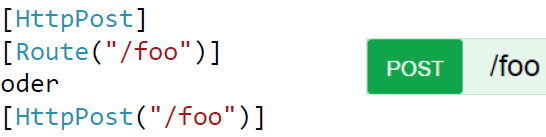
\includegraphics{asp_routing_1.png}
\end{minipage}
\begin{minipage}{0.5\linewidth}
  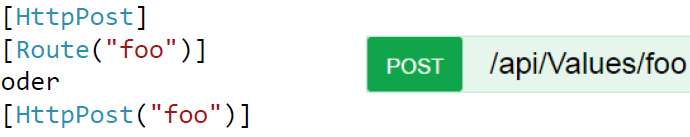
\includegraphics{asp_routing_2.png}
\end{minipage}
\subsection{Sonstiges}
\textcolor{b}{\textbf{Swagger:}} Eine Spezifikation für die Dokumentation von REST APIs. Programmiersprachen unabhängig. Wird im \textit{Startup.cs} eingetragen. Default unter \textit{http://[server-name]/swagger} erreichbar. \textcolor{b}{\textbf{REST HATEOAS:}} Verlinkte Daten als Links zu Verfügung stellen. \textcolor{b}{\textbf{Exception Handling:}} Error Handling soll generisch funktionieren. $\rightarrow$ Vorgehen: Es gibt eine Exception, welche die notwendigen Daten sammelt. Es gibt einen globalen Errorhandler, welcher diese Exception für Client aufbereitet. Bei einem ungültigen Zustand wird Custom-Exception ausgelöst.
